	\documentclass[10pt,oneside]{CBFT_book}
	% Algunos paquetes
	\usepackage{amssymb}
	\usepackage{amsmath}
	\usepackage{graphicx}
	\usepackage{libertine}
	\usepackage[bold-style=TeX]{unicode-math}
	\usepackage{lipsum}

	\usepackage{natbib}
	\setcitestyle{square}

	\usepackage{polyglossia}
	\setdefaultlanguage{spanish}
	



	\usepackage{CBFT.estilo} % Cargo la hoja de estilo

	% Tipografías
	% \setromanfont[Mapping=tex-text]{Linux Libertine O}
	% \setsansfont[Mapping=tex-text]{DejaVu Sans}
	% \setmonofont[Mapping=tex-text]{DejaVu Sans Mono}

	%===================================================================
	%	DOCUMENTO PROPIAMENTE DICHO
	%===================================================================

\begin{document}

% =================================================================================================
\chapter{Introducción}
% =================================================================================================


% =================================================================================================
\section{El experimento de Stern-Gerlach}
% =================================================================================================

Un horno emite átomos de plata (Ag) neutros con un electrón $e$ en la última órbita que le da el spín
al átomo como un todo. Al salir del horno los átomos tienen su spín orientado en cualquier dirección.
Ver figura.
El momento magnético del átomo que sale del horno es 
\[
	\vb{mu} = \frac{e}{m_e c} \vb{S}
\]

\begin{figure}[htb]
	\begin{center}
	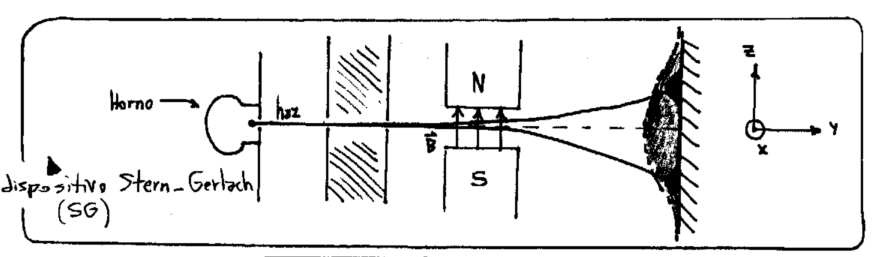
\includegraphics[width=0.8\textwidth]{images/teo2_1.pdf}	 
	\end{center}
	\caption{}
\end{figure} 

La fuerza $f_z$ que le ejerce el campo \vb{B} a estos átomos es 
\[
	f_z \propto - \mu_z
\]
de modo que el dispositivo SG mide y filtra por $S_z(\mu_z)$. Si el spín es un ente clásico
es de esperar un patrón como el sombreado en azul, pero se obtienen dos manchas; con la
correspondencia mostrada bajo estas líneas
\begin{figure}[htb]
	\begin{center}
	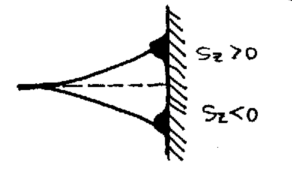
\includegraphics[width=0.4\textwidth]{images/teo2_2.pdf}	 
	\end{center}
	\caption{}
\end{figure} 

Entonces el spín no es un ente {\it continuo}: está cuantizado y sólo puede tomar dos valores.
Llamamos a estos estados
\[
	(S_z,+) \qquad \qquad (S_z,-)
\]
Luego, un aparato de SG filtra o selecciona ciertos átomos. Podemos combinarlos.

\begin{figure}[htb]
	\begin{center}
	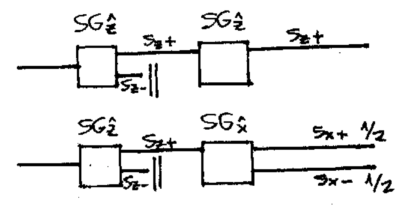
\includegraphics[width=0.4\textwidth]{images/teo2_3.pdf}	 
	\end{center}
	\caption{}
\end{figure} 

Con el dispositivo segundo orientado en $\hat{x}$ obtenemos mitad de átomos en
$(S_z,+)$ y mitad en $(S_z,-)$. La única es que en realidad lo que sucede es que 
$(S_z,+)$ se compone de $(S_x,+)$ y $(S_x,-)$.

Acá abajo sale $(S_z,-)$ pero para que ello sea posible 
$(S_x,+)$ se debe componer de $(S_z,+)$ y $(S_z,-)$. Pero esto no es posible
porque al segundo aparato no entró jamás $(S_z,-)$. Se filtró antes.

Los spines en 

\begin{figure}[htb]
	\begin{center}
	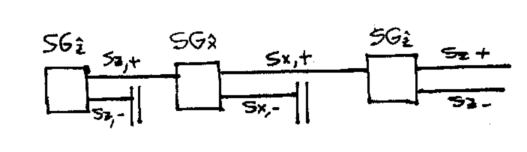
\includegraphics[width=0.4\textwidth]{images/teo2_4.pdf}	 
	\end{center}
	\caption{}
\end{figure} 



% \bibliographystyle{CBFT-apa-good}	% (uses file "apa-good.bst")
% \bibliography{CBFT.Referencias} % La base de datos bibliográfica

\end{document}
